\documentclass[12pt]{article}
\usepackage{amsmath,amsfonts,fullpage,amsthm,graphicx}

\newtheorem*{theorem}{Theorem}
\newtheorem*{fact}{Fact}
\newtheorem*{goal}{Goal}
\newtheorem*{idea}{Idea}
\newtheorem*{defn}{Definition}
\newtheorem*{ex}{Example}

%Style section
%\setlength{\textheight}{10in}
%\setlength{\textwidth}{7in}
%\hoffset=-0.75in
 \pagestyle{plain}
% \setlength{\topmargin}{0in}
% \setlength{\headsep}{0in}
% \setlength{\oddsidemargin}{0in}
% \setlength{\evensidemargin}{0in}

\begin{document}


\pagestyle{empty} %use this to get rid of page numbers

\noindent
{Math 166 \hskip 1.5 truein  Names:\ \hrulefill}

\noindent
%\vskip 0.3truein
%\bigskip
%\noindent
{Arc length, surface area, and pressure}

\noindent \hskip 3.5 truein  Section Number:\ \hrulefill
\medskip

\begin{goal} \rm
Apply integration to calculate arc length, surface area, and fluid pressure.
\end{goal}
%\smallskip

\begin{enumerate}
\item What is the formula for calculating the arc length of a curve? Describe the main idea behind how we derived this formula.
\vspace{1in}


\item Show that the arc length of $f(x)=x^{3/2}$ from $x=0$ to $x=1$ equals $\frac{13\sqrt{13}-8}{27}$.



\vspace{3.25in}

%\item $\displaystyle\int 4x (\ln x)^2\ dx$

%\item Write an integral for the {arc length} of the curve $y=\frac{1}{4}x^4$ over the interval $[1,2]$. Instead of evaluating the integral exactly, approximate this integral using the trapezoidal rule with $n=5$. What is the error bound for this approximation?  $\mbox{Error}(T_n)\leq \displaystyle\frac{K_2 (b-a)^3}{12 n^2}$.


%\vspace{3in}

\item  What is the formula for the surface area of a surface of revolution formed by rotating the graph $y=f(x)$ for $a\leq x\leq b$ about the $x$-axis? Describe the main idea behind how we derived this formula.

\vspace{1in}


\pagebreak
\item Find the surface area of the surface of revolution created by rotating the graph $y=x^3$ for $0\leq x\leq 1$ about the $x$-axis.


\vspace{3.75in}

%\item Use Simpson's rule with $n=6$ to {approximate} the surface area of the surface obtained by rotating the curve $y=\ln(x)$ for $1\leq x\leq 3$ about the $x$-axis. What is the error bound for this approximation? $\mbox{Error}(S_n)\leq \frac{K_4 (b-a)^5}{180 n^4}$ where $|f^{(4)}(x)|\leq K_4 \mbox{ for } a\leq x\leq b$.


\newpage 


\begin{align*}
	\sin^2(x)&=\frac{1-\cos(2x)}{2}\\
	\cos^2(x)&=\frac{1+\cos(2x)}{2}\\
\end{align*}


\item  A circular window on a submarine has a radius of 2 meters, and the center of the window is 8 meters below water level. Write and evaluate an integral to calculate the fluid force on the window by using the diagram below.
%Recall fluid force equals $\rho g \int y f(y) \ dy$ where $f(y)$ is the width of the window at $y$. Also r
Recall the density of water is 1000 $kg/m^3$ and the acceleration due to gravity is $g=9.8 ~m/s^2$. 

\smallskip
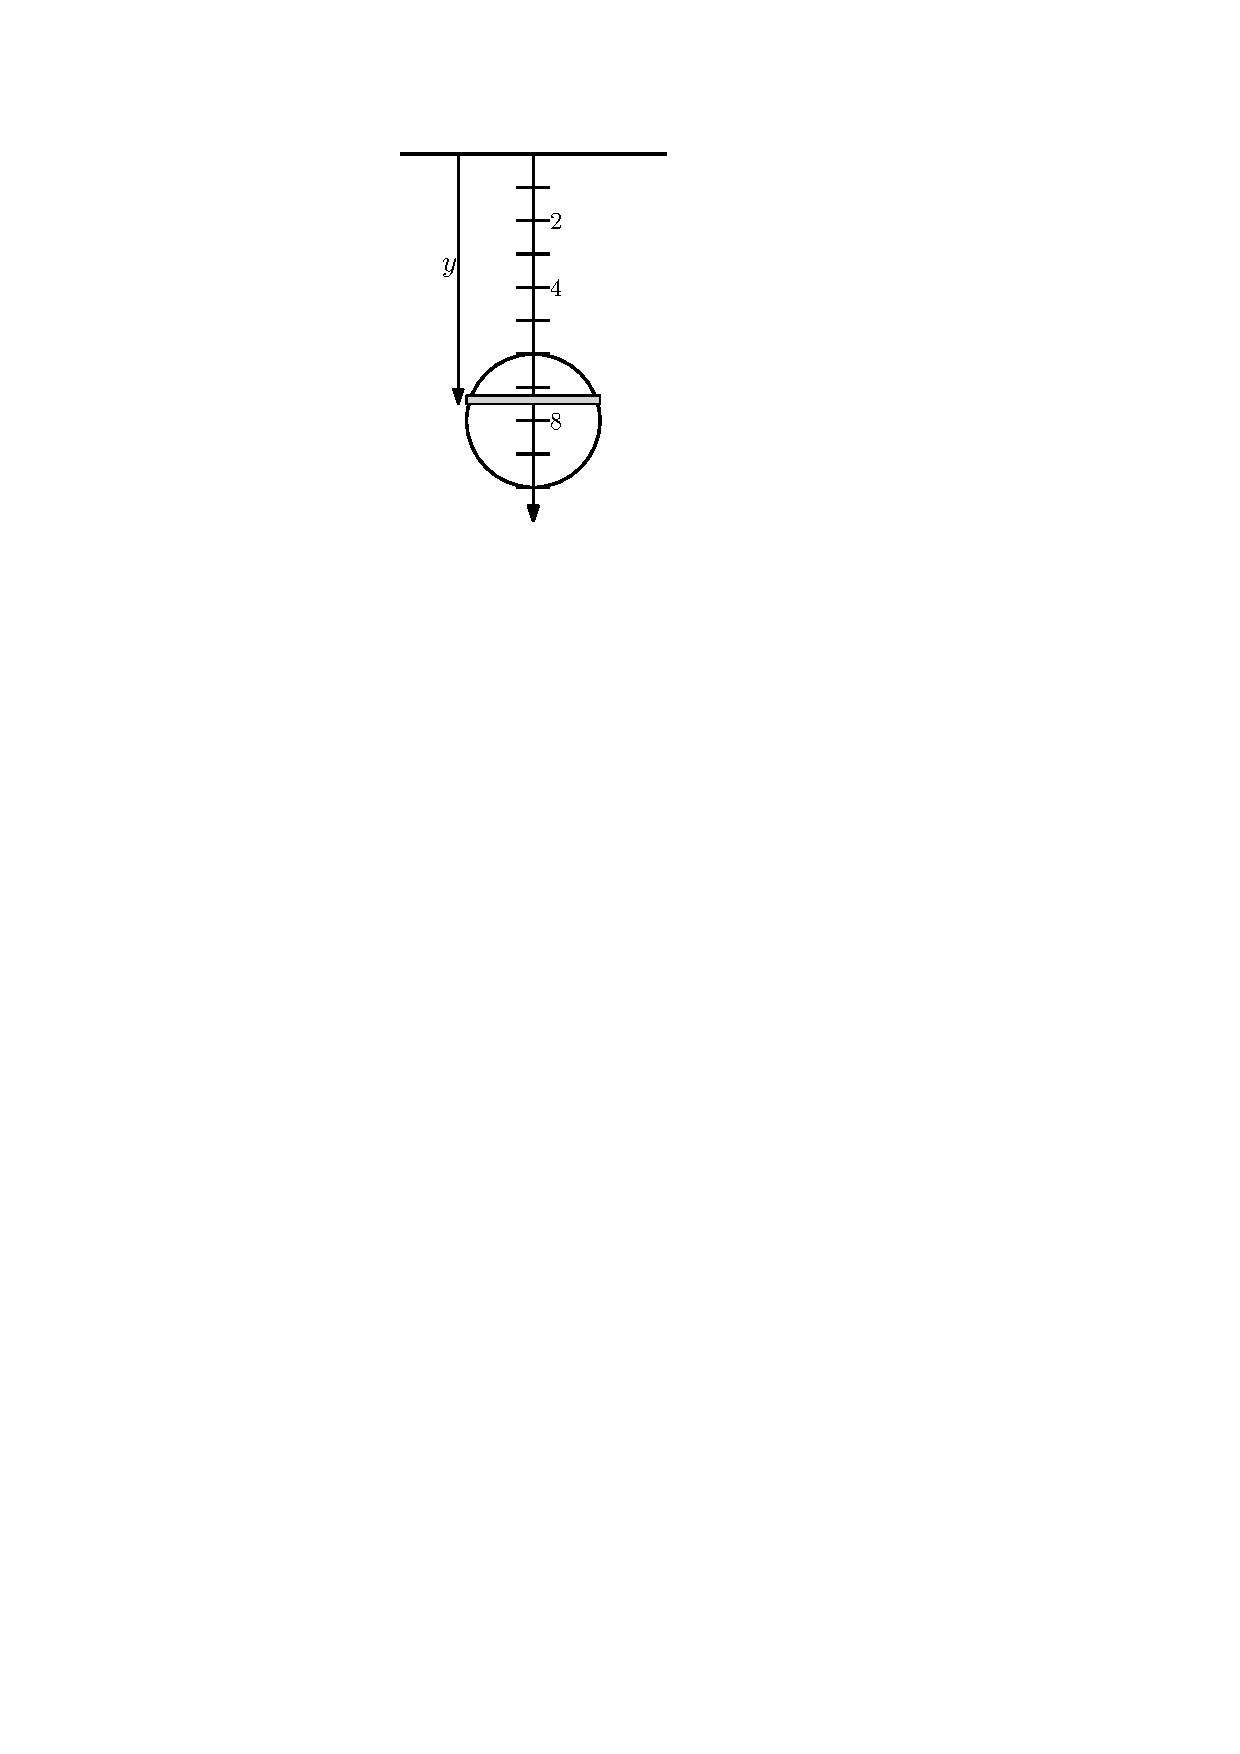
\includegraphics[scale=.75]{circle_depth_no_eq}

\bigskip

\bigskip

Note it may be easier to evaluate the integral if you set up your axes with the point $(0,0)$ in the middle of the circle, as below. In this case, the depth no longer equals $y$; you need to figure out an expression for the depth at $y$.  Write another integral expressing the fluid force on the window by using the diagram below.  Verify that these integrals are equivalent.


\bigskip

\bigskip
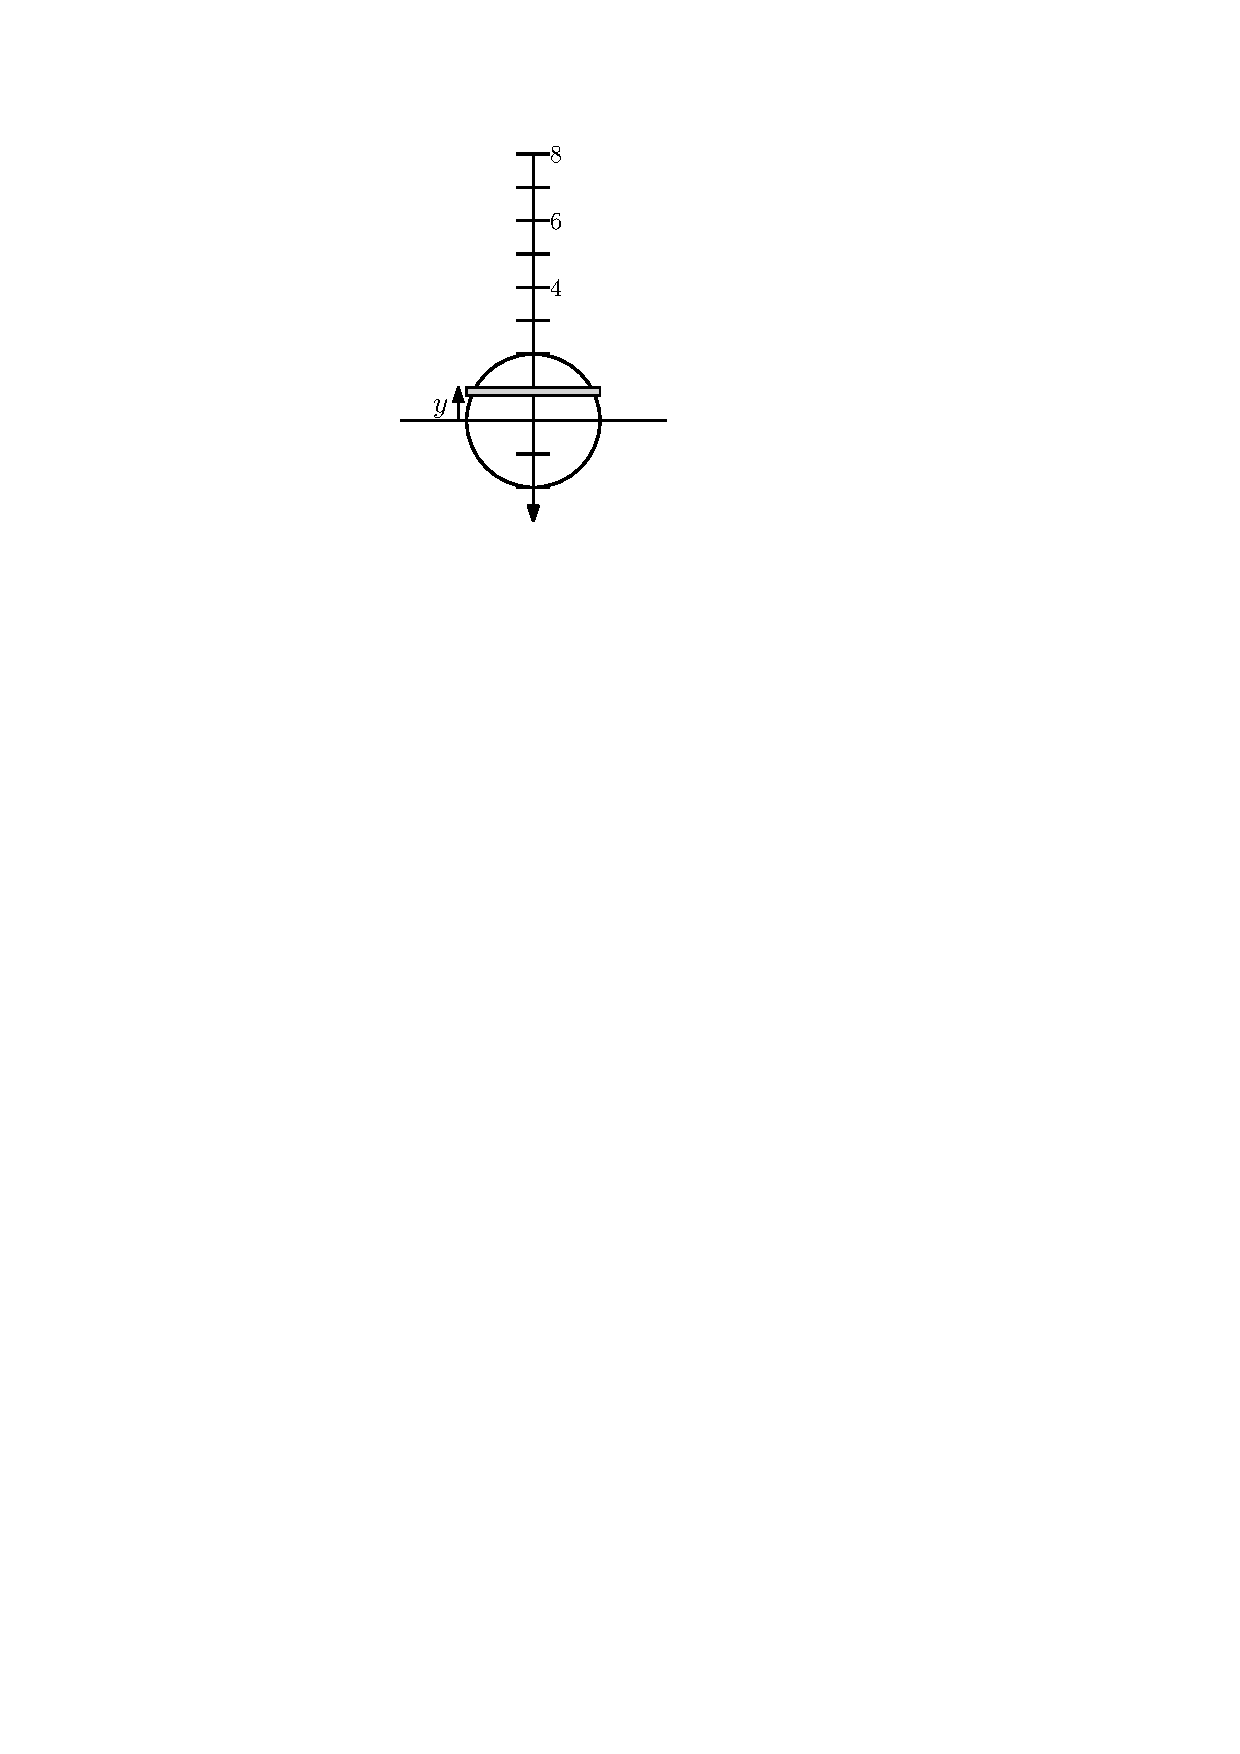
\includegraphics[scale=.75]{circle_depth2_no_eq}

%\item Show that the center of mass of a system of point masses $m_1=6$, $m_2=3$, $m_3=2$, $m_4=9$ located at $(3,-2)$, $(0,0)$, $(-5,3)$, and $(4,2)$, respectively, is $\left(\frac{11}{5},\frac{3}{5}\right)$.
%
%\vspace{2in}
%
%\item Find the center of mass $(\bar{x},\bar{y})$ of a thin lamina of uniform density $\delta$ bounded by the graph of $f(x)=4-x^2$ and the $x$-axis. %Recall $\bar{x}=\frac{M_y}{M}$ and $\bar{y}=\frac{M_x}{M}$. 
%Hint: you can use symmetry to determine $\bar{x}$ without even calculating an integral!
%\vspace{2.3in}
%
%\item Show that the center of mass, or centroid, of a thin lamina of uniform density $\delta$ bounded by the graphs of $f(x)=4-x^2$ and $g(x)=x+2$ is $\left(\frac{-1}{~2},\frac{12}{5}\right)$.

%\pagebreak
%\vspace{3in}

\end{enumerate} 

\end{document}
